% Asset ID: AS1AlgebraicExpressionsTIKZ-002
% Source: CCEA AS1-AF-LO001 and Dr Frost index laws examples
% Related lesson section: Core Theory, Worked Examples, Exam Technique
% Purpose: Present the core index laws as a compact rule card.

\documentclass[tikz,border=8pt]{standalone}
\usetikzlibrary{positioning}

\begin{document}
\begin{tikzpicture}[
    font=\sffamily,
    row/.style={draw, thick, minimum height=0.85cm, anchor=west},
    head/.style={draw, thick, fill=black, text=white, font=\sffamily\bfseries, minimum height=0.85cm, anchor=west},
    note/.style={draw, rounded corners=4pt, thick, fill=gray!8, align=left, text width=13.4cm}
]

\node[font=\sffamily\bfseries\Large, anchor=west] at (0,0) {Index laws for rational exponents};
\node[font=\sffamily\small, anchor=west] at (0,-0.45) {Use the law only when the structure matches. Same-base laws need the same base.};

\def\xA{0}
\def\xB{4.2}
\def\xC{8.2}
\def\xD{12.1}
\def\wA{4.2}
\def\wB{4.0}
\def\wC{3.9}
\def\wD{3.3}

\node[head, minimum width=\wA cm] at (\xA,-1.25) {Situation};
\node[head, minimum width=\wB cm] at (\xB,-1.25) {Law};
\node[head, minimum width=\wC cm] at (\xC,-1.25) {Example};
\node[head, minimum width=\wD cm] at (\xD,-1.25) {Move};

\node[row, minimum width=\wA cm] at (\xA,-2.10) {Same base multiplication};
\node[row, minimum width=\wB cm] at (\xB,-2.10) {$a^m a^n=a^{m+n}$};
\node[row, minimum width=\wC cm] at (\xC,-2.10) {$x^3x^2=x^5$};
\node[row, minimum width=\wD cm] at (\xD,-2.10) {add indices};

\node[row, fill=gray!5, minimum width=\wA cm] at (\xA,-2.95) {Same base division};
\node[row, fill=gray!5, minimum width=\wB cm] at (\xB,-2.95) {$\dfrac{a^m}{a^n}=a^{m-n}$};
\node[row, fill=gray!5, minimum width=\wC cm] at (\xC,-2.95) {$\dfrac{x^3}{x^2}=x$};
\node[row, fill=gray!5, minimum width=\wD cm] at (\xD,-2.95) {subtract indices};

\node[row, minimum width=\wA cm] at (\xA,-3.80) {Power of a power};
\node[row, minimum width=\wB cm] at (\xB,-3.80) {$(a^m)^n=a^{mn}$};
\node[row, minimum width=\wC cm] at (\xC,-3.80) {$(x^3)^2=x^6$};
\node[row, minimum width=\wD cm] at (\xD,-3.80) {multiply indices};

\node[row, fill=gray!5, minimum width=\wA cm] at (\xA,-4.65) {Power of a product};
\node[row, fill=gray!5, minimum width=\wB cm] at (\xB,-4.65) {$(ab)^n=a^nb^n$};
\node[row, fill=gray!5, minimum width=\wC cm] at (\xC,-4.65) {$(4x^3y)^3=64x^9y^3$};
\node[row, fill=gray!5, minimum width=\wD cm] at (\xD,-4.65) {power to each factor};

\node[row, minimum width=\wA cm] at (\xA,-5.50) {Zero power};
\node[row, minimum width=\wB cm] at (\xB,-5.50) {$a^0=1,\ a\ne0$};
\node[row, minimum width=\wC cm] at (\xC,-5.50) {$7^0=1$};
\node[row, minimum width=\wD cm] at (\xD,-5.50) {non-zero base};

\node[row, fill=gray!5, minimum width=\wA cm] at (\xA,-6.35) {Negative power};
\node[row, fill=gray!5, minimum width=\wB cm] at (\xB,-6.35) {$a^{-m}=\dfrac{1}{a^m}$};
\node[row, fill=gray!5, minimum width=\wC cm] at (\xC,-6.35) {$3^{-2}=\dfrac19$};
\node[row, fill=gray!5, minimum width=\wD cm] at (\xD,-6.35) {reciprocal};

\node[row, minimum width=\wA cm] at (\xA,-7.20) {Fractional power};
\node[row, minimum width=\wB cm] at (\xB,-7.20) {$a^{m/n}=(\sqrt[n]{a})^m$};
\node[row, minimum width=\wC cm] at (\xC,-7.20) {$32^{2/5}=4$};
\node[row, minimum width=\wD cm] at (\xD,-7.20) {root, then power};

\node[note] at (7.55,-8.35)
{\textbf{Exam trap:} Do not add indices when collecting like terms. For example, $10x^3+x^3=11x^3$, not $11x^6$.};

\end{tikzpicture}
\end{document}
